\chapter{Methods}

The sizes of meteors are determined through a long chain of physical relations that begin with its apparent magnitude. So, first thing to do is be able to find the magnitude of the fireball when D6 detects it. We have written a script where we can find the magnitude of the fireball as long as we know the apparent magnitude of an object in the sky, such as a star. This is done through automatically centering on the brightest part of the region near the place the user clicks on the image, and then automatically detecting the edges of the  object through the creation of a fitting centroid. A Gaussian curve is then fitted to its light curve to integrate over and extract the value of all its pixels. This summation of pixels gives us the raw magnitude for our specific camera. The general outline can be seen in Figure~\ref{fig:flowchart}.

\begin{figure}[htpb]
	\centering
	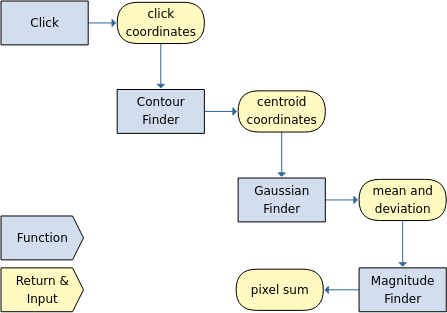
\includegraphics[width=.8\linewidth]{Flow.png}
	\caption{A visual guide of the script.}
	\label{fig:flowchart}
\end{figure}

\section{Photometry}

Once an event is detected by D6, it can then be run through a script that will analyze the frames and output the desired photometric information. The script is written in Python 3, and the user can run it through the use of the accompanying graphic user interface. The interface can be seen in Figure~\ref{fig:gui}. A user simply runs the script while directing it to the location of the video they would like to analyze. The program runs through the video a single frame at a time, and loops through its functions until completing all the frames in the video.

\begin{figure}[htpb]
	\centering
	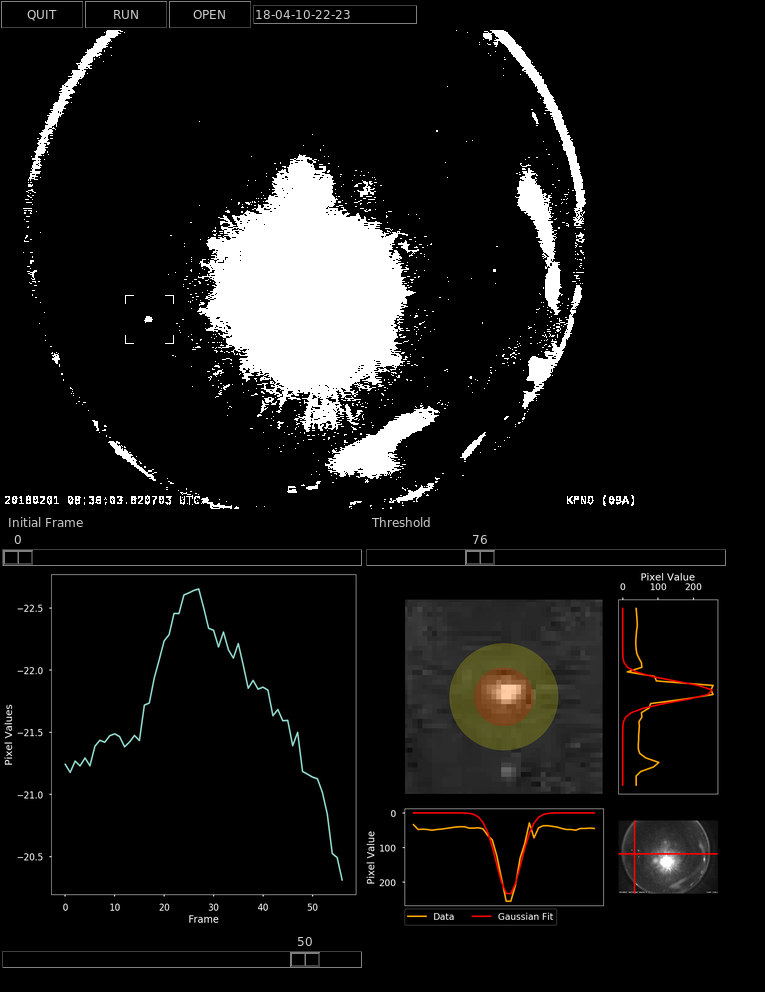
\includegraphics[width=0.6\linewidth]{gui.png}
	\caption{The GUI allows one to see the initial frame, and view the results all in one window.}
	\label{fig:gui}
\end{figure}
Upon running the script, the user will first see the first frame of the video. This is where the user will be required to make a selection on the screen identifying where the object and reference stars are located. The user simply left clicks on the desired object, and right clicks on a reference star of known magnitude. An example of a frame that a user could see is seen in Figure~\ref{fig:scene}. The user clicks initialize the script. 

\begin{figure}[ht!]
	\centering
	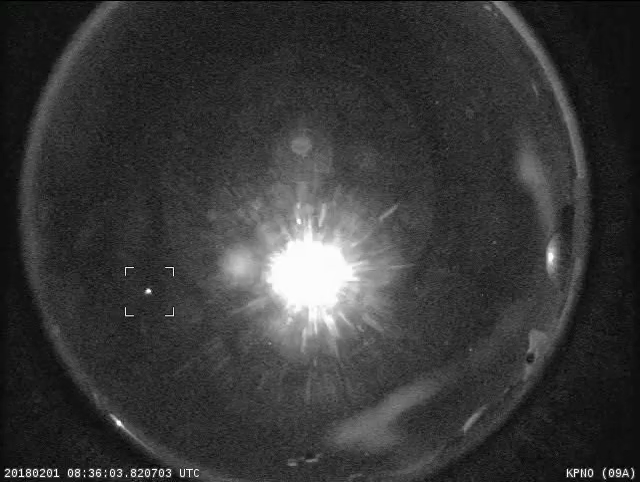
\includegraphics[width=0.6\linewidth]{scene.png}
	\caption{The first frame of an event. The user clicks on this image in the GUI.}
	\label{fig:scene}
\end{figure}

\subsection{Recognizing a User's Click}

The program needs a general idea of where the object is in question on the frame. It can follow the moving object after that, as long as it has a starting point. The user provides this starting point by identifying the object they're concerned about, along with the star they want to use as reference. This is outlined in Figure~\ref{fig:clickfinder}

\begin{figure}[h!]
	\centering
	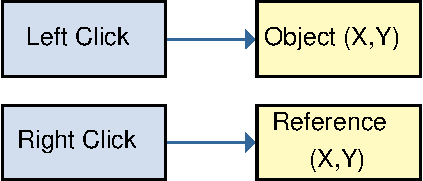
\includegraphics[width=0.6\linewidth]{clickfinder.pdf}
	\caption{The purpose of the initial clicking by the user.}
	\label{fig:clickfinder}
\end{figure}

Using the \texttt{OpenCV} computer vision python package, the coordinates of the user's clicks can be extracted and used in the script. The user's left click records the corresponding X and Y coordinates as a tuple identify as the location of the object. The user's right click records the corresponding tuple as the location of the reference star. The user can click multiple times, with each click overwriting the previous one until the user is satisfied with their click accuracy. They exit this stage of the program with a key press.

%The location of the center of the object is done through the use of two functions: a \texttt{click} function and a \texttt{FindingMax} function. The click function allows the user to interact with the image through OpenCV. The function creates two global variables that are crucial to the activation of the other following functions: The x and y coordinates of that click. After all, without the user clicking to identify the object and the reference star, the program has nothing to analyse. These variables are tuples containing the x and y positions that were clicked. In order to differentiate the reference star and the object, different clicks were assigned to each one. A left click marks the coordinates as the location of the reference star, and a right click will mark the coordinates as the location of the fireball. The program will only record the latest clicks when the image is open; previous clicks will be overridden by the newest clicks. The program does not continue until the user exits the frame window with a key press.

\subsection{Fitting a contour to the object}
The location of the object is now identify as the exact pixel the user clicked on. The user may have provided a solid estimate on where that is with their click, but it most likely not the true center. This estimate is enough for the program, as it can now run its algorithm to find a more accurate location of the object. This more accurate object location will be necessary when the program tries to fit Gaussian fits to the data, which will be needed to identify the radius of the object. This process is outlined in Figure~\ref{fig:contourfinder}.

\begin{figure}[h!]
	\centering
	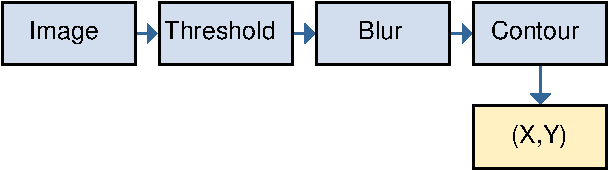
\includegraphics[width=\linewidth]{contourfinder.pdf}
	\caption{The steps the image is process with to get a more accurate object position}
	\label{fig:contourfinder}
\end{figure}

The script takes the X and Y coordinates of where the user thinks the object is and isolates that part of the frame. The image is then blurred using an \texttt{OpenCV} command that blurs the edges of the pixels using a Gaussian equation to fade their light. This is done as the sharp edges of pixels next to each other are not ideal to model a continuous equation off of. The image is then thresholded at a certain percentage. Thresholding essentially divides all pixels into a group lighter than the percentage and a group darker than the percentage. The darker pixels are all turned black, and the lighter pixels are all turned white. This, combined with the blurring, turns the object into a white ellipse. An example of this thresholding can be seen in Figure~\ref{fig:nothresholdd6}, which is a thresholded version of Figure~\ref{fig:thresholdd6}. 

\begin{figure}[ht!]
	\centering
	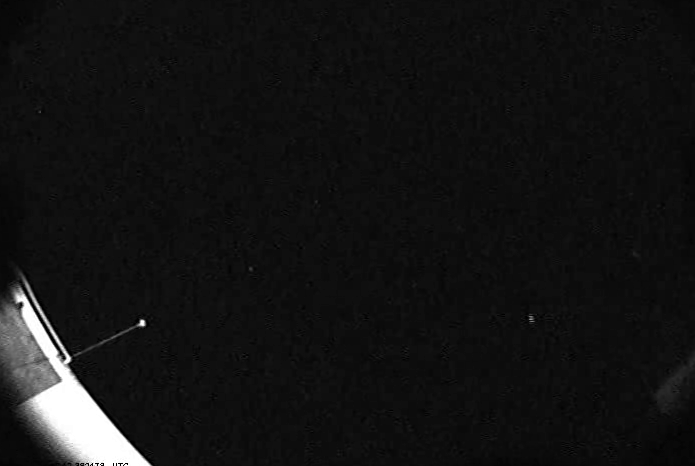
\includegraphics[width=0.5\linewidth]{thresholdd6.png}
	\caption{The fireball in a unaltered frame can sometimes be too dim for the program to detect for the entirety of the event.}
	\label{fig:nothresholdd6}
\end{figure}

\begin{figure}[ht!]
	\centering
	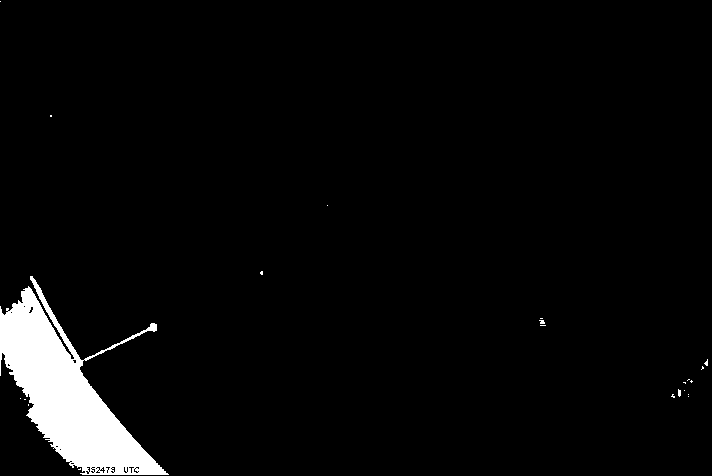
\includegraphics[width=0.5\linewidth]{nothresholdd6.png}
	\caption{A thresholded image, when adjusted properly, allows the program to locate an object easier.}
	\label{fig:thresholdd6}
\end{figure}

This process also has the benefit of making it easier for the user to locate the object. It is especially useful for finding the reference star, which is often much dimmer than the meteor. This is evident by no stars being visible in Figure~\ref{fig:thresholdd6}, but some being visible in Figure~\ref{fig:nothresholdd6}.

Another OpenCV command called \texttt{findContours} is implemented to find the center of that ellipse. Its algorithm is exactly like how one would find the center of mass of an object, but with the intensity of the object being the "mass" in the calculations. The created ellipse has a clear circle shape it can work with, and it finds the center with that. At this point, the program now has the known center to a much more precise degree. With the objects coordinates updated, the thresholded frame is discarded, and the following analysis is continued with the undoctored data. 


\subsection{Fitting a Gaussian to the contour}
Now that there is an accurate object location, we can fit a Gaussian curve to the data in both the X and Y dimensions. We want to do this because having a Gaussian curve gives us a known standard deviation, and we can then calculate the radius of the object using that standard deviation. This process is outlined in Figure~\ref{fig:gaussianfinder}.

\begin{figure}[h!]
	\centering
	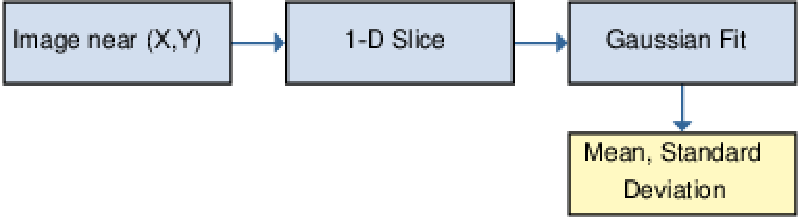
\includegraphics[width=\linewidth]{gaussianfinder.pdf}
	\caption{The steps taken to find the Gaussian parameters of the data.}
	\label{fig:gaussianfinder}
\end{figure}

The formula for a Gaussian curve is 

\begin{equation}
	ae^{(-(x-x_0)^2/(2\sigma^2))}
\end{equation}
where a is the amplitude, $x_0$ is the point along the curve, and $\sigma$ is the standard deviation. A function is used from the Python library called \texttt{SciPy}footnote{The author prefers the package to be pronounced "skip-ee" when discussing any matter involving this paper}. A Gaussian function will output a mean and standard deviation, but first the \texttt{SciPy} function needs a strong estimate of the mean to attempt to fit the data. This is why the center of the object was calculated using the contour method previous discussed. In our program, we calculate two one-dimensional Gaussian curves across that center. The function fits the Gaussian curves to 20 pixel slices centered at the point in the X and Y directions. The Gaussian curve also returns its mean, and the mean of X slice and the Y slice is updated to represent the objects location once again. The last three functions can be thought of as a sequence of steps to acquire the most accurate center, along with the acquisition of the standard deviation data mentioned. The curves can be plotted and saved as PNGs. The Gaussian curves of one such frame can be  seen in Figure~\ref{fig:testplot}.

\begin{figure}[h!]
	\centering
	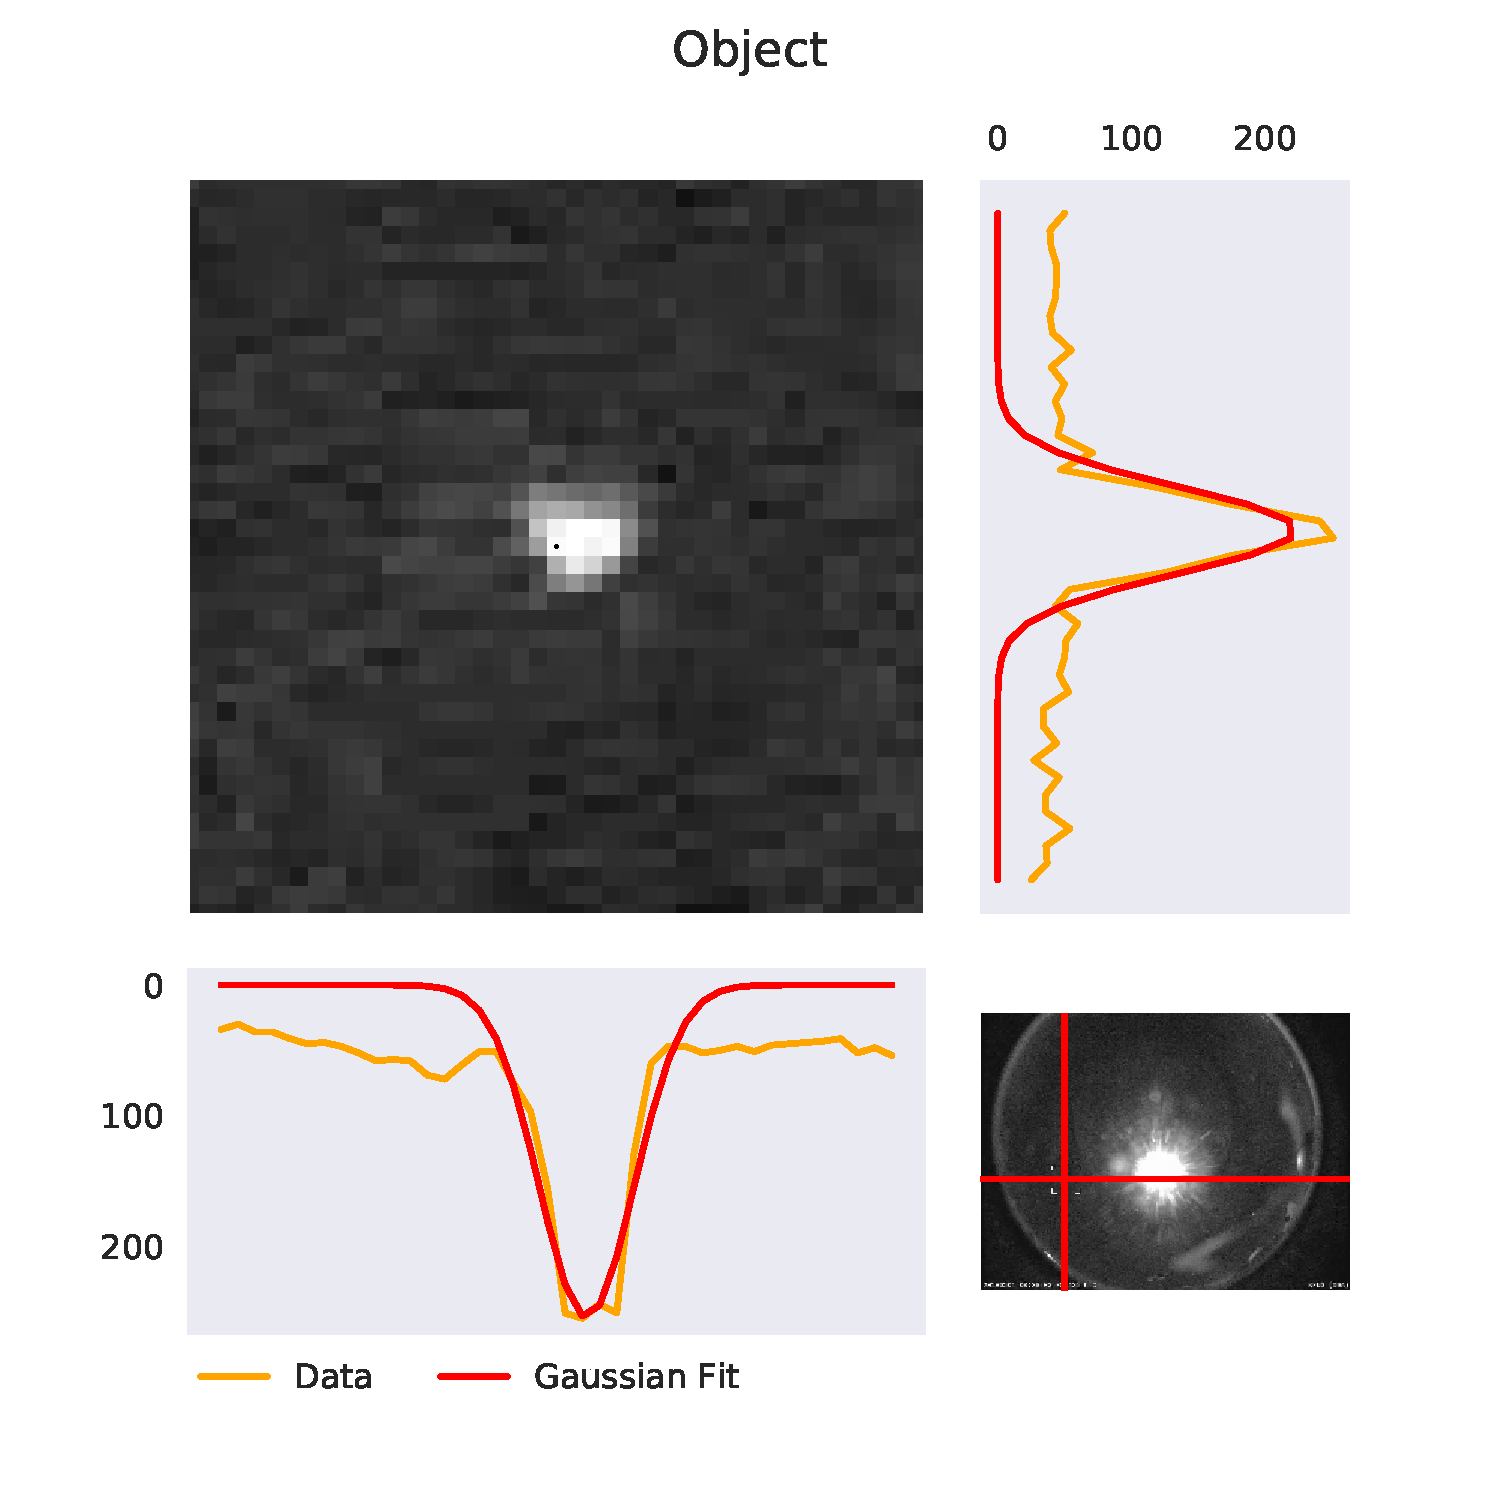
\includegraphics[width=.6\linewidth]{testplot.pdf}
	\caption{The Gaussian curves in this plot align with the image, so one can visually confirm that they are fitting the data.}
	\label{fig:testplot}
\end{figure}



Occasionally, an anomaly or poor data will make the Gaussian function unable to actually fit the data to a Gaussian curve. In this case, an exception is called in the code to just use the estimates provided as the true outputs of the Gaussian function instead of the error message. The frame is skipped in the creation of the final light curve. This is done to ensure the program can finish to completion, and not end in the middle. Later on, it is possible to view the data to ensure the Gaussian curves aligned well with the pixel values.


A Gaussian curve is to be expected from something such as a point light source; it dims out radially. An object will not have a definite edge: it will fade away into the background. This can be shown in Figure~\ref{fig:NoCircles} of a Gaussian fit. Gaussian function has the benefit that it's percentage of light is directly related to the number of standard deviations. This is commonly known as the 68-95-99.7 rule: one standard deviation covers 68\% of the data, two standard deviations covers 95\% of the data, and three standard deviations covers 99.7\% of the data. After that, the diminishing returns are not enough to overcome the extra noise in our data. 

\begin{figure}[ht!]
	\centering
	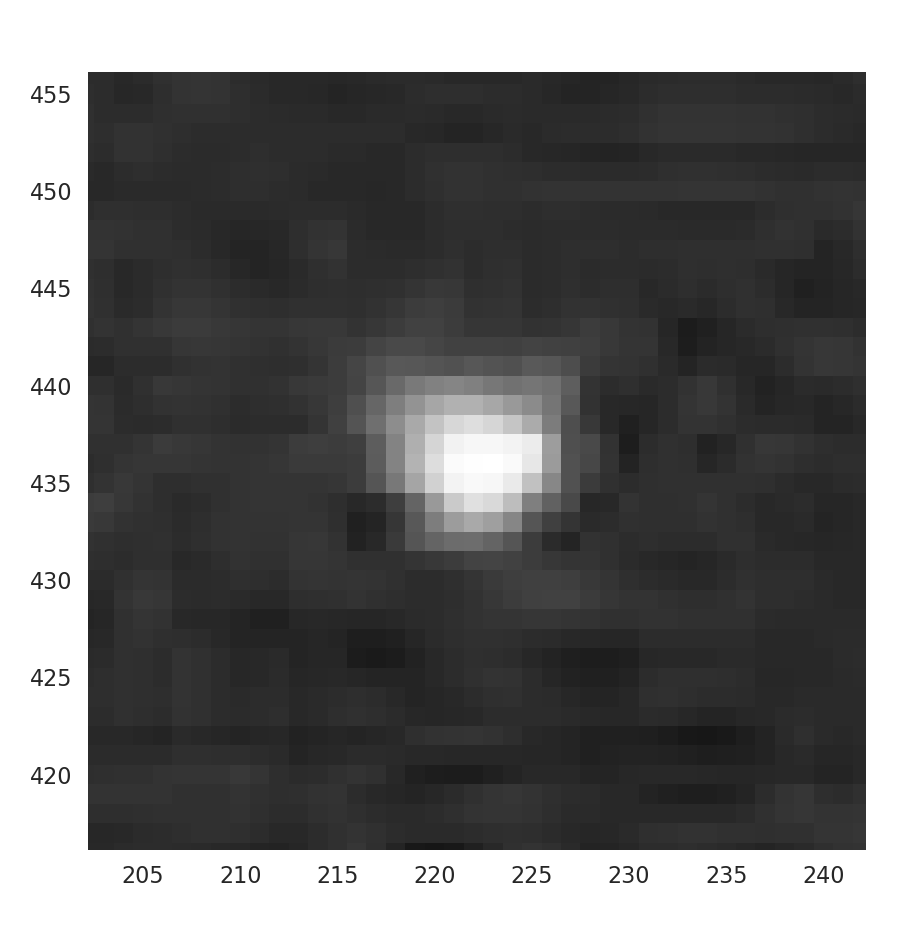
\includegraphics[width=.4\linewidth]{NoCircles.png}
	\caption{The object is located in the center of this slice, and its light fades radially out from that center.}
	\label{fig:NoCircles}
\end{figure}

\subsection{Calculating the magnitude of the object}

Now all of the needed information is gathered to find the magnitude of the object at that frame. With the parameters from the Gaussian function, we know where the object is centered and, by defining its radius to be two standard deviations, we know the radius of the object. After subtracting background light, we then can sum over all the pixels within that radius to find the amount of light, or the magnitude, that our camera sees from the object.  Doing this every frame gives us the light curve of the event over time. This process can be seen in Figure~\ref{fig:magfinder}.

\begin{figure}[htpb]
	\centering
	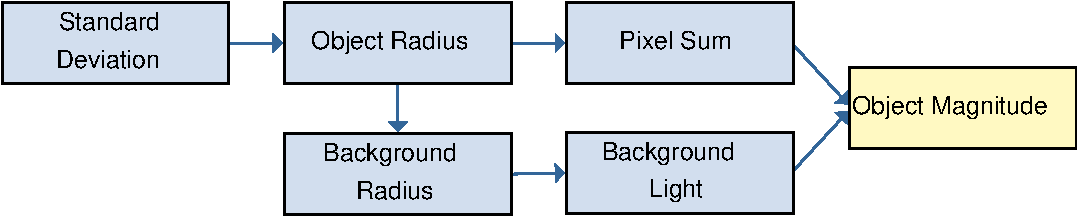
\includegraphics[width=\linewidth]{magfinder.pdf}
	\caption{The steps the function goes through to find the magnitude of the object.}
	\label{fig:magfinder}
\end{figure}


There are few details in the calculation of the radius from the standard deviations, however. The X and Y radii are defined by multiplying their respective Gaussian curve standard deviations by two, and then rounding up to the nearest integer. While the standard deviations themselves may be decimals, the image consists of only integer values, so any other number would not be compatible. In other words, one can not sum over a fraction of a pixel; either the entire pixel is used or none of it is. The radius of the circle is then defined to be whichever of these two radii happen to be the largest. They should be the same in theory, but may vary by a pixel due to the rounding process mentioned. 

The radius can give us the lengths along the axis, but not the pixels of the entire circle we are searching over. The program takes a 10 x 10 search area around the center point, and checks all the points to see if they lie inside the given radius using the distance formula. If a point is within the radius, it is appended to a list to be used later. This can be seen in Figure~\ref{fig:radius}

\begin{figure}[ht!]
	\centering
	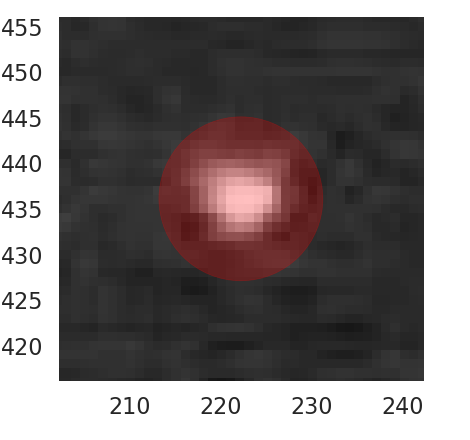
\includegraphics[width=0.4\linewidth]{Radius.png}
	\caption{The pixels in red are within the calculated radius for this fireball.}
	\label{fig:radius}
\end{figure}

We need to remove the background light from the calculation so we can sum over the pixel values attributed to the object's light only, not from any other source. If the background light is not subtracted the values of the pixels would be artificially elevated due to the existence of that inherent background light. To do this, we need to find a second radius of points around the circle that can be used to determine the average value of the background light. The background light can be somewhat noisy, so that is why we take an average of a group of background pixels. The pixels in question are chosen by finding pixels within a radius of the object's radius + 10 pixels, not including the pixels inside the object's radius. This creates a ring around the object's radius, as shown in Figure~\ref{fig:background}

\begin{figure}[ht!]
	\centering
	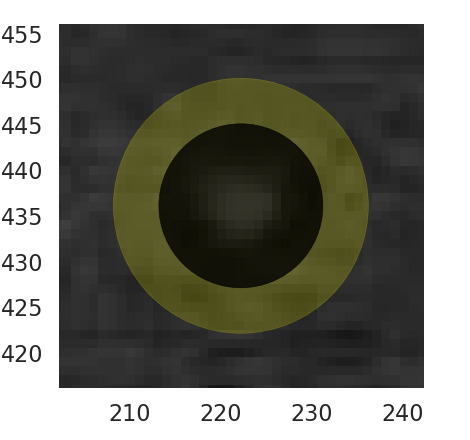
\includegraphics[width=0.4\linewidth]{BackgroundRing.png}
	\caption{The pixels in yellow are the values being used to find the average background value. The object can be seen inside the yellow ring.}
	\label{fig:background}
\end{figure}

One problem that occasionally happens is the background search radius will go beyond the actual size of the image. This problem occurs when an object gets close to the sides of the image. In order to prevent this, and crashing the program, a loop goes through the pixel indices in the background list and checks to make sure they are not greater than the dimensions of the image. If any are, they are ignored. 

There is also a one pixel buffer between the two areas for extra wiggle room. This is important due to the conversion to integers when finding the two radii. The radii are not perfect circles, as while the distance may be in the middle of a pixel, you can not just split a pixel. Both of the radii calculations round up, and take that whole pixel, which could create a pixel on the edge of the background radius and the object radius being used in both summations if there was not a buffer zone.This is easily seen when both the object's radius and the background ring is displayed on the same picture, such as in Figure~\ref{fig:BothCircles} 

\begin{figure}[ht!]
	\centering
	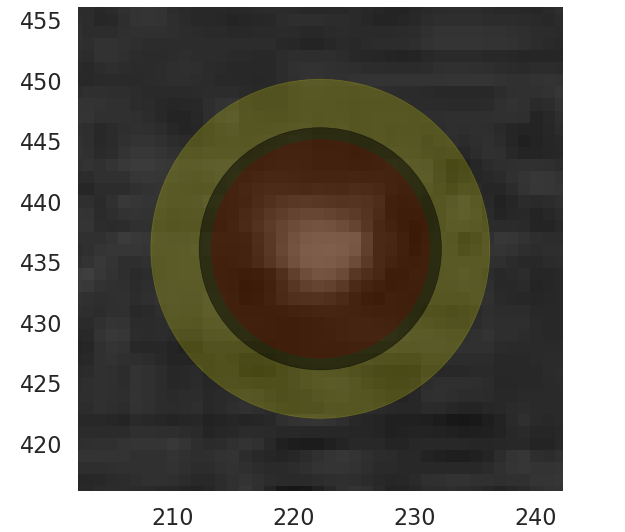
\includegraphics[width=0.4\linewidth]{BothCircles.png}
	\caption{The pixels in orange are within the object's radius. The yellow pixels are the background ring. The gray area in-between is the buffer.}
	\label{fig:BothCircles}
\end{figure}

The program then sums all the pixel values in the list of values that were within the inner radius. This is done through a for loop that adds the value onto itself with every iteration through the list, while subtracting the average background magnitude from each individual point. This is the raw measurement of light from that specific camera.

Cameras have different sensitivities, so there is an offset that needs to be accounted for to have our specific camera be able to align with the standard units of magnitude.   This is then entered into Equation~\ref{equation:instrument} to find the instrumental magnitude. 

\begin{equation}
	M_I = -2.5 \log_{10}\left( \sum \text{pixels}\right) + \text{offset}
	\label{equation:instrument}
\end{equation}

This is the same equation from the previous section. The offset can be calculated by Equation~ref{equation:instrument}

\begin{equation}
	\text{offset} = M_I - M_C
	\label{equation:offset}
\end{equation}
where $M_I$ and $M_C$ are the instrumental magnitudes and catalog magnitudes of the same object.

This is why a reference star is needed. The object in question, the fireball, does not have a catalog magnitude, but the reference star does. This calculates the offset for the camera, which then can be applied to equation~\ref{equation:offset} for the fireball. This offset is calculated as an average over the entire event. This is because the small amount of fluctuation each frame may have in their offsets due to variables such as atmospheric distortion or haze is much less than the noise that exists from the use of one one-thirtieth second frame as calibration.

The program does runs the previously mentioned functions for every frame in the video, and loops through this process until the video is completed. This overview can be seen in Figure~\ref{\fig:moreflow}.

\begin{figure}[ht!]
	\centering
	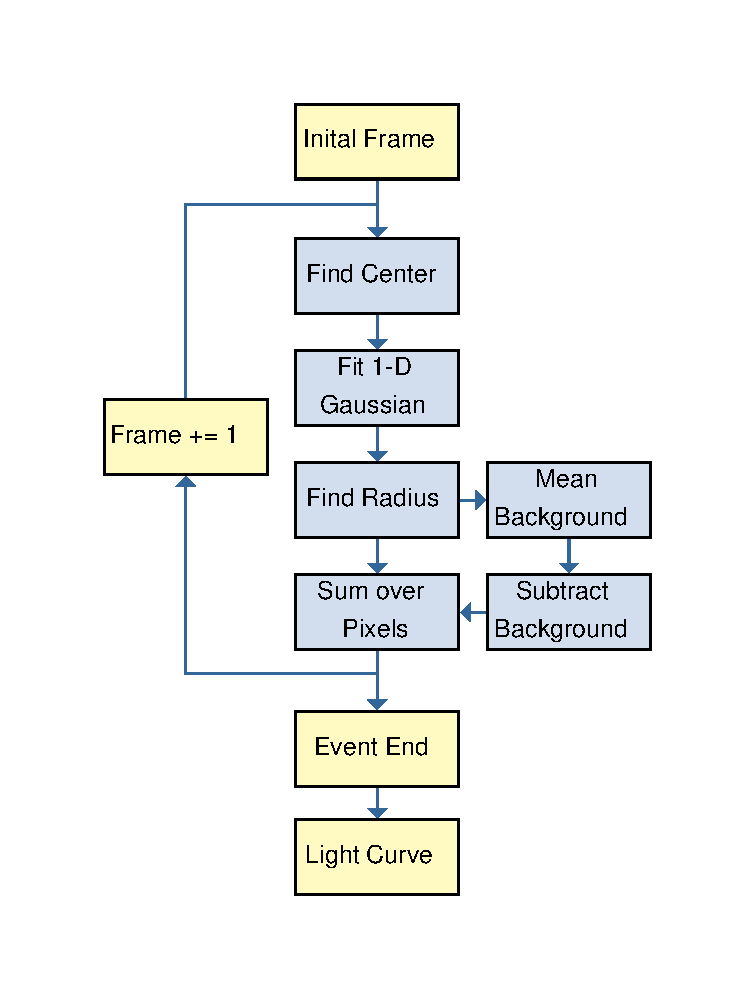
\includegraphics[width=\linewidth]{flowchart.pdf}
	\caption{Flowchart}
	\label{fig:moreflow}
\end{figure}

The process of calculating a more precise center through each step allows the program to adjust the previous frame's center to the next frame's center without any difficulty, as the amount of pixels the center of the object appears to travel in each frame is within the margin of error of the original estimates at the beginning of the program. This process is shown in Figure~\ref{\fig:updatingxy}

\begin{figure}[htpb]
	\centering
	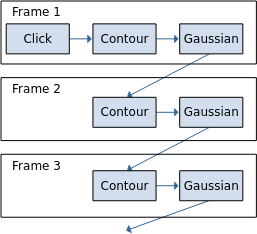
\includegraphics[width=0.5\linewidth]{updatingxy.png}
	\caption{The updating process of the values used as the object's coordinates}
	\label{fig:updatingxy}
\end{figure}

The video processing is done through using the video read functionality of \texttt{OpenCV}. The video frames are always converted to grayscale at the beginning of the loop, so there is only one channel of pixel values instead of three that would occur with color video.  PNGs of each frame's Gaussian fits along with the visualization of the radii are optional through the loop. If enabled, the result is exactly like Figure~\ref{fig:testplot}. If this is enabled, the program may take up to 30 seconds to run, as it is memory intensive to save hundreds of PNGs. If it is disabled, the program finishes within a second.




